\documentclass[tikz]{standalone}
\usepackage{pgfplots}
\pgfplotsset{compat=1.15}
\usepackage{mathrsfs}
\usetikzlibrary{arrows,calc}
\usepackage{tkz-euclide}
\pagestyle{empty}

\definecolor{AngleClr}{rgb}{0,0.39215686274509803,0}
\definecolor{ShapeClr}{rgb}{0.6,0.2,0}

\begin{document}

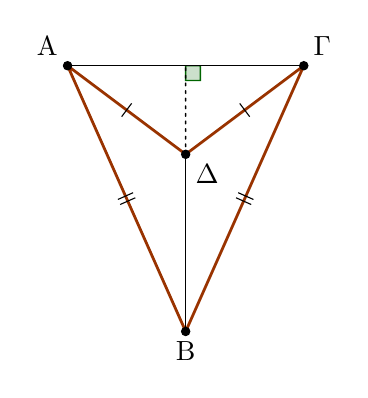
\begin{tikzpicture}[scale=.75]
\tkzSetUpLine[line width=1pt,color=black]
\tkzSetUpPoint[fill=black]

\tkzDefPoints{0/0/A,4/0/C,2/-1.5/D,2/-4.5/B}

\tkzFillPolygon[fill=white](A,B,C,D)

% Find the intersection of the diagonals.
\tkzInterLL(B,D)(A,C) \tkzGetPoint{I}

\tkzMarkRightAngle[line width=0.5pt, size=.25,color=AngleClr,fill=AngleClr,fill opacity=0.2](D,I,C)

\tkzDrawSegments[line width=0.5pt,color=black](A,C B,D)
\tkzDrawSegments[line width=0.5pt,color=black,dashed,dash pattern=on 1pt off 1.75pt](D,I)

\tkzDrawPolygon[color=ShapeClr](A,B,C,D)
\tkzDrawPoints[size=3](A,B,C,D)
\tkzLabelPoint[above left](A){$\rm A$}
\tkzLabelPoint[below](B){$\rm B$}
\tkzLabelPoint[above right](C){$\rm \Gamma$}
\tkzLabelPoint[below right](D){$\rm \Delta$}

\tkzMarkSegments[mark=|,size=3](D,A D,C)
\tkzMarkSegments[mark=||,size=3](B,A B,C)

\end{tikzpicture}

\end{document}
